%!TEX root = ../ausarbeitung.tex
\newpage
\section{Klassifizierung mit Histograms of Gradients und Support Vector Machines} \label{sec:HOG}


\subsection{Einführung zu Histograms of Oriented Gradients} \label{ssec:intro_HOG}

Die Bezeichnung \textit{Histograms of Oriented Gradients} (HOG) bezeichnet einen Feature Deskriptor und wurde bekannt durch die Arbeit von Navneet Dalal und Bill Triggs \cite{dalal05}. Diese setzen den HOG-Deskriptor ein um Fußgänger zu detektieren. Später wurde er auch für andere Objekte eingesetzt. Die Berechnung des HOG-Deskriptors lässt sich in drei Schritte unterteilen: Gradientenberechnung, Gruppierung der Orientierungen und Histogrammerzeugung. Häufig werden  auch Vorverarbeitungsschritte, wie zum Beispiel ein Histogrammausgleich durchgeführt.

Zur Gradientenberechnung wird der Sobel-Operator verwendet. Eine visuelle Darstellung des Ergebnisses ist in Abbildung~\ref{fig:sobel} gezeigt. Zu sehen ist die Magnitude der Ableitung über die vertikale (links) und horizontale (rechts) Bildachse. Dabei entspricht in dieser Darstellung der Grauwert der positiv definierten Magnitude des Gradienten. Mit den folgenden Formeln lassen sich aus den beiden Gradientenbildern die positiv definierte gesamt Magnitude $|G|$ und die Orientierung $\Theta$ berechnen:  

\begin{equation}
|G| = \sqrt{G_x^2 + G_y^2}
\end{equation}
\begin{equation}
\Theta = \arctan({G_x, G_y})
\end{equation}

\begin{center}
\begin{tabular}{c}
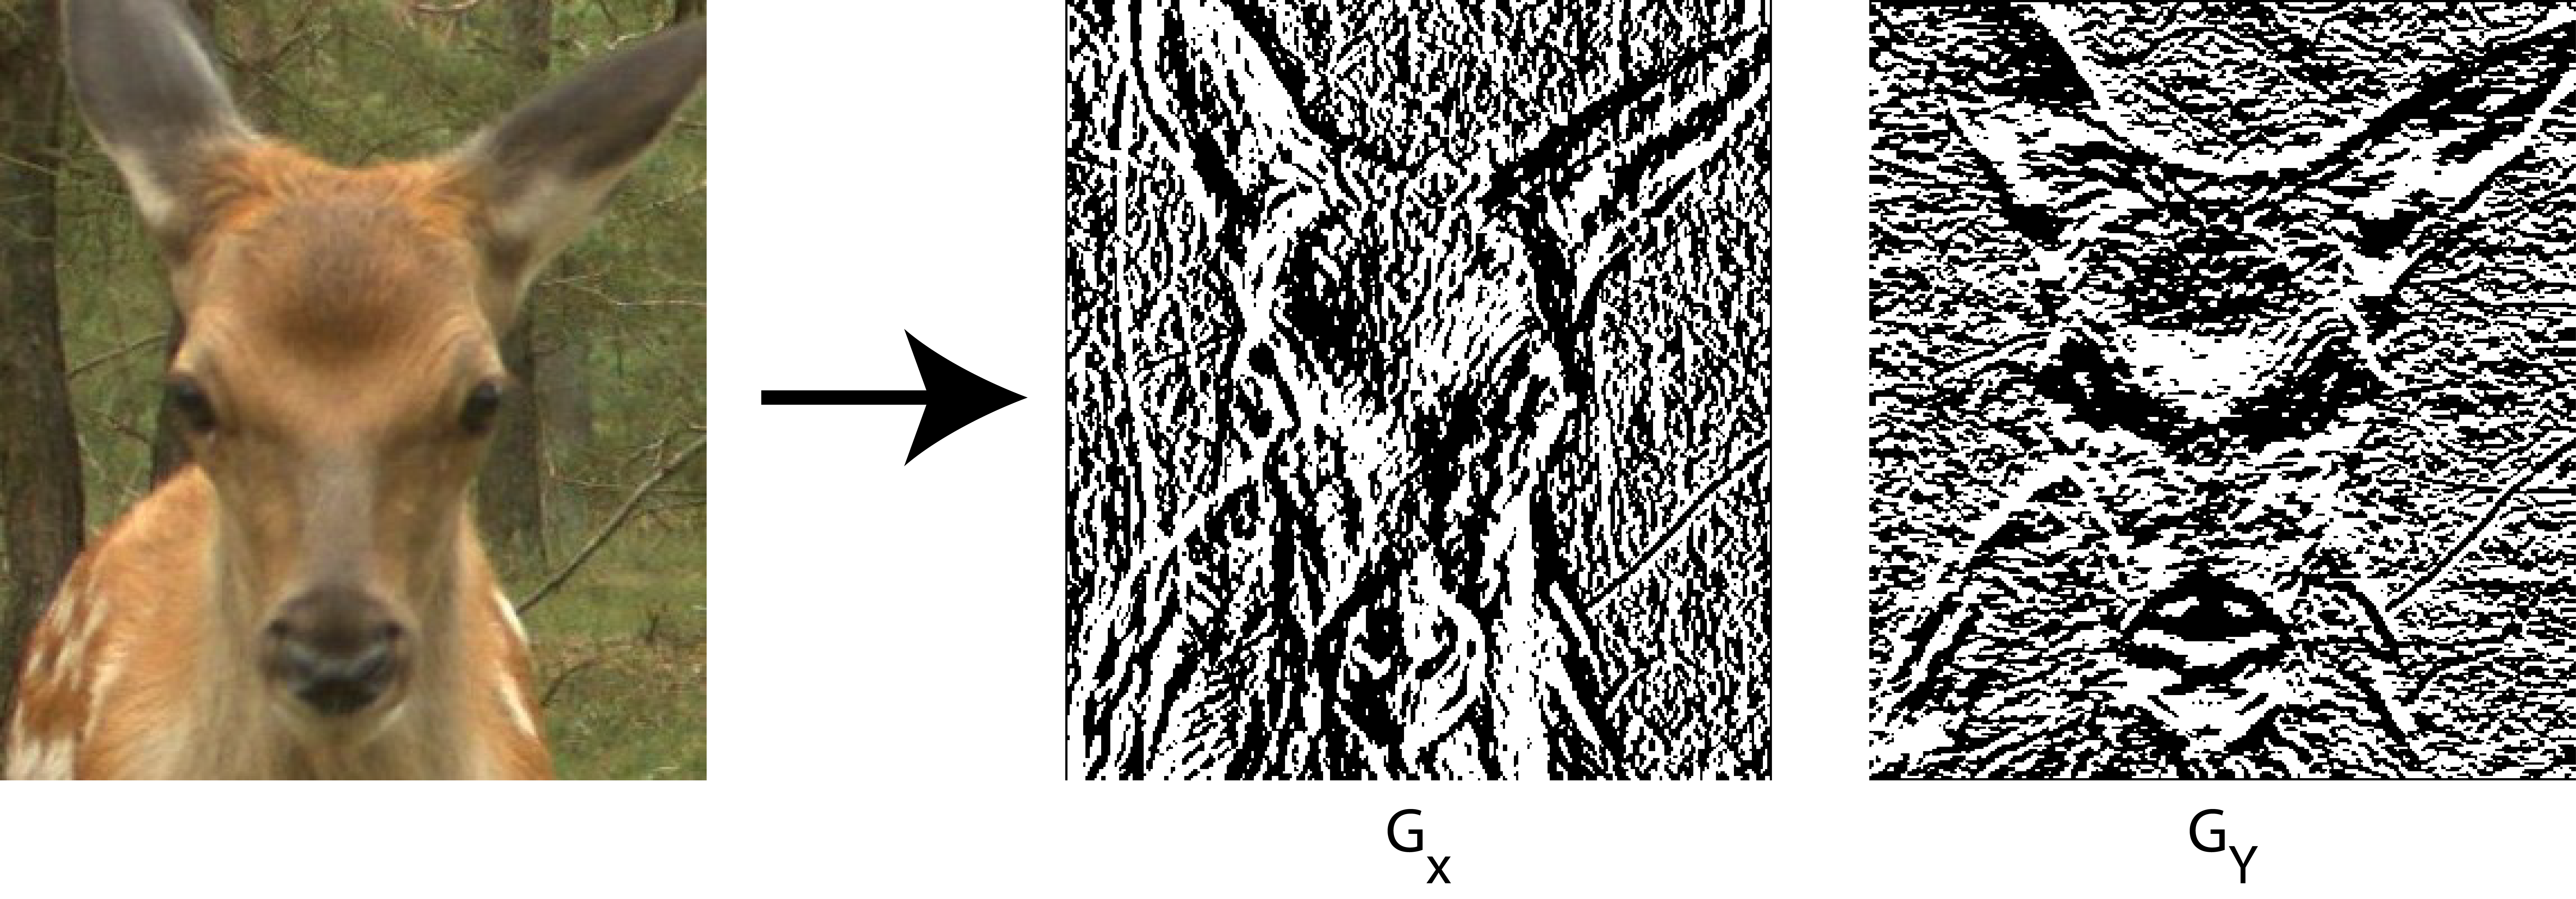
\includegraphics[trim={0 0cm 0cm 0cm},clip=true,width=13cm]{img/sobel.png}
\end{tabular}
\captionof{figure}{Exemplarische Ergebnisbilder des Sobel-Operators für die vertikale und horizontale Bildachse. Die Grauwerte entsprechen der Magnitude des Gradienten.}
\label{fig:sobel}
\end{center}

Für jeden Pixel eines Bildes wird die Magnituden und Orientierung berechnet. Anschließend werden sie entsprechend ihrer Orientierung in Gruppen sortiert. Häufig wird die Richtung der Orientierung ignoriert und 9 Gruppen verwendet. Durch das Ignorieren der Richtung wird also nur ein halber Kreis betrachtet (0 - 180°). Bei 9 Gruppen bedeutet dies, dass jede Gruppe 20° abdeckt. Der Wert dieser Gruppe ist dann die Summe aller Magnituden der Pixel, die dieser Gruppe zugewiesen wurden. Es ist jedoch auch möglich andere Einteilungen zu verwenden. 
Formal ist ein solche Histogramm aus 9 Werten bereits ein HOG. Allerdings ist der Informationsgehalt dieser Repräsentation sehr gering. Um den Informationsgehalt zu erhöhen wird das Bild stattdessen systematisch in gleich große Bereiche unterteilt und für jeden Bereich ein Histogramm gebildet. Diese Histogramme werden abschließend konkateniert und als ein HOG-Deskriptor verwendet. Durch die Unterteilung werden Informationen der einzelnen Bildbereiche bewahrt und die räumliche Struktur des Bilds kann wesentlich besser beschrieben werden. Die systematische Unterteilung des Bildes wird wir folgt durchgeführt. Das Bild wird in gleich große Zellen unterteilt, so das jedes Pixel in genau einer Zelle enthalten ist (siehe Abbildung~\ref{fig:sobel2hog} rotes Raster). Anschließend werden jeweils vier dieser Zellen zu einem Block zusammengefasst (siehe Abbildung~\ref{fig:sobel2hog} grünes Rechteck) und für jeden dieser Blöcke wird nach dem \textit{Sliding Window} Prinzip eine Histogramm erstellt. Jedes dieser Histogramm wird anschließend normalisiert um eine belichtungsunabhängige Repräsentation zu erhalten. Dies bedeutet das jede Zelle, außer den Randzellen, vier mal in einem Histogramm repräsentiert wird. Dies führt dazu, dass durch die Normalisierung, alle lokalen Kontexte betrachtet werden und weniger Information durch die Normalisierung verloren geht. So wird zum Beispiel die Invarianz zu Schatten im Bild erhöht. 
Exemplarisch ist in Abbildung~\ref{fig:img2HOG} eine visuell aufbereitete Repräsentation eines HOG-Deskriptors gezeigt. In dieser Darstellung ist das gezeigte Reh noch zu erkennen, da der Deskriptor deutlich die Kanten des Tieres hervorhebt. Diese veranschaulicht, dass die essentiellen Informationen erhalten bleiben obwohl die Datenmenge auf einen Bruchteil reduziert wurde. Um die Vergleichbarkeit der HOG-Deskriptoren zu gewährleisten muss garantiert werden, dass die Deskriptoren die selbe Dimension besitzen. Dies wird erreicht, indem die betrachteten Bilder oder Bildausschnitte auf eine einheitliche Größe skaliert werden und anschließend das selbe Raster aus Zellen verwendet wird.  \cite{dalal05}\cite{HOG1}
\begin{center}
\begin{tabular}{c}
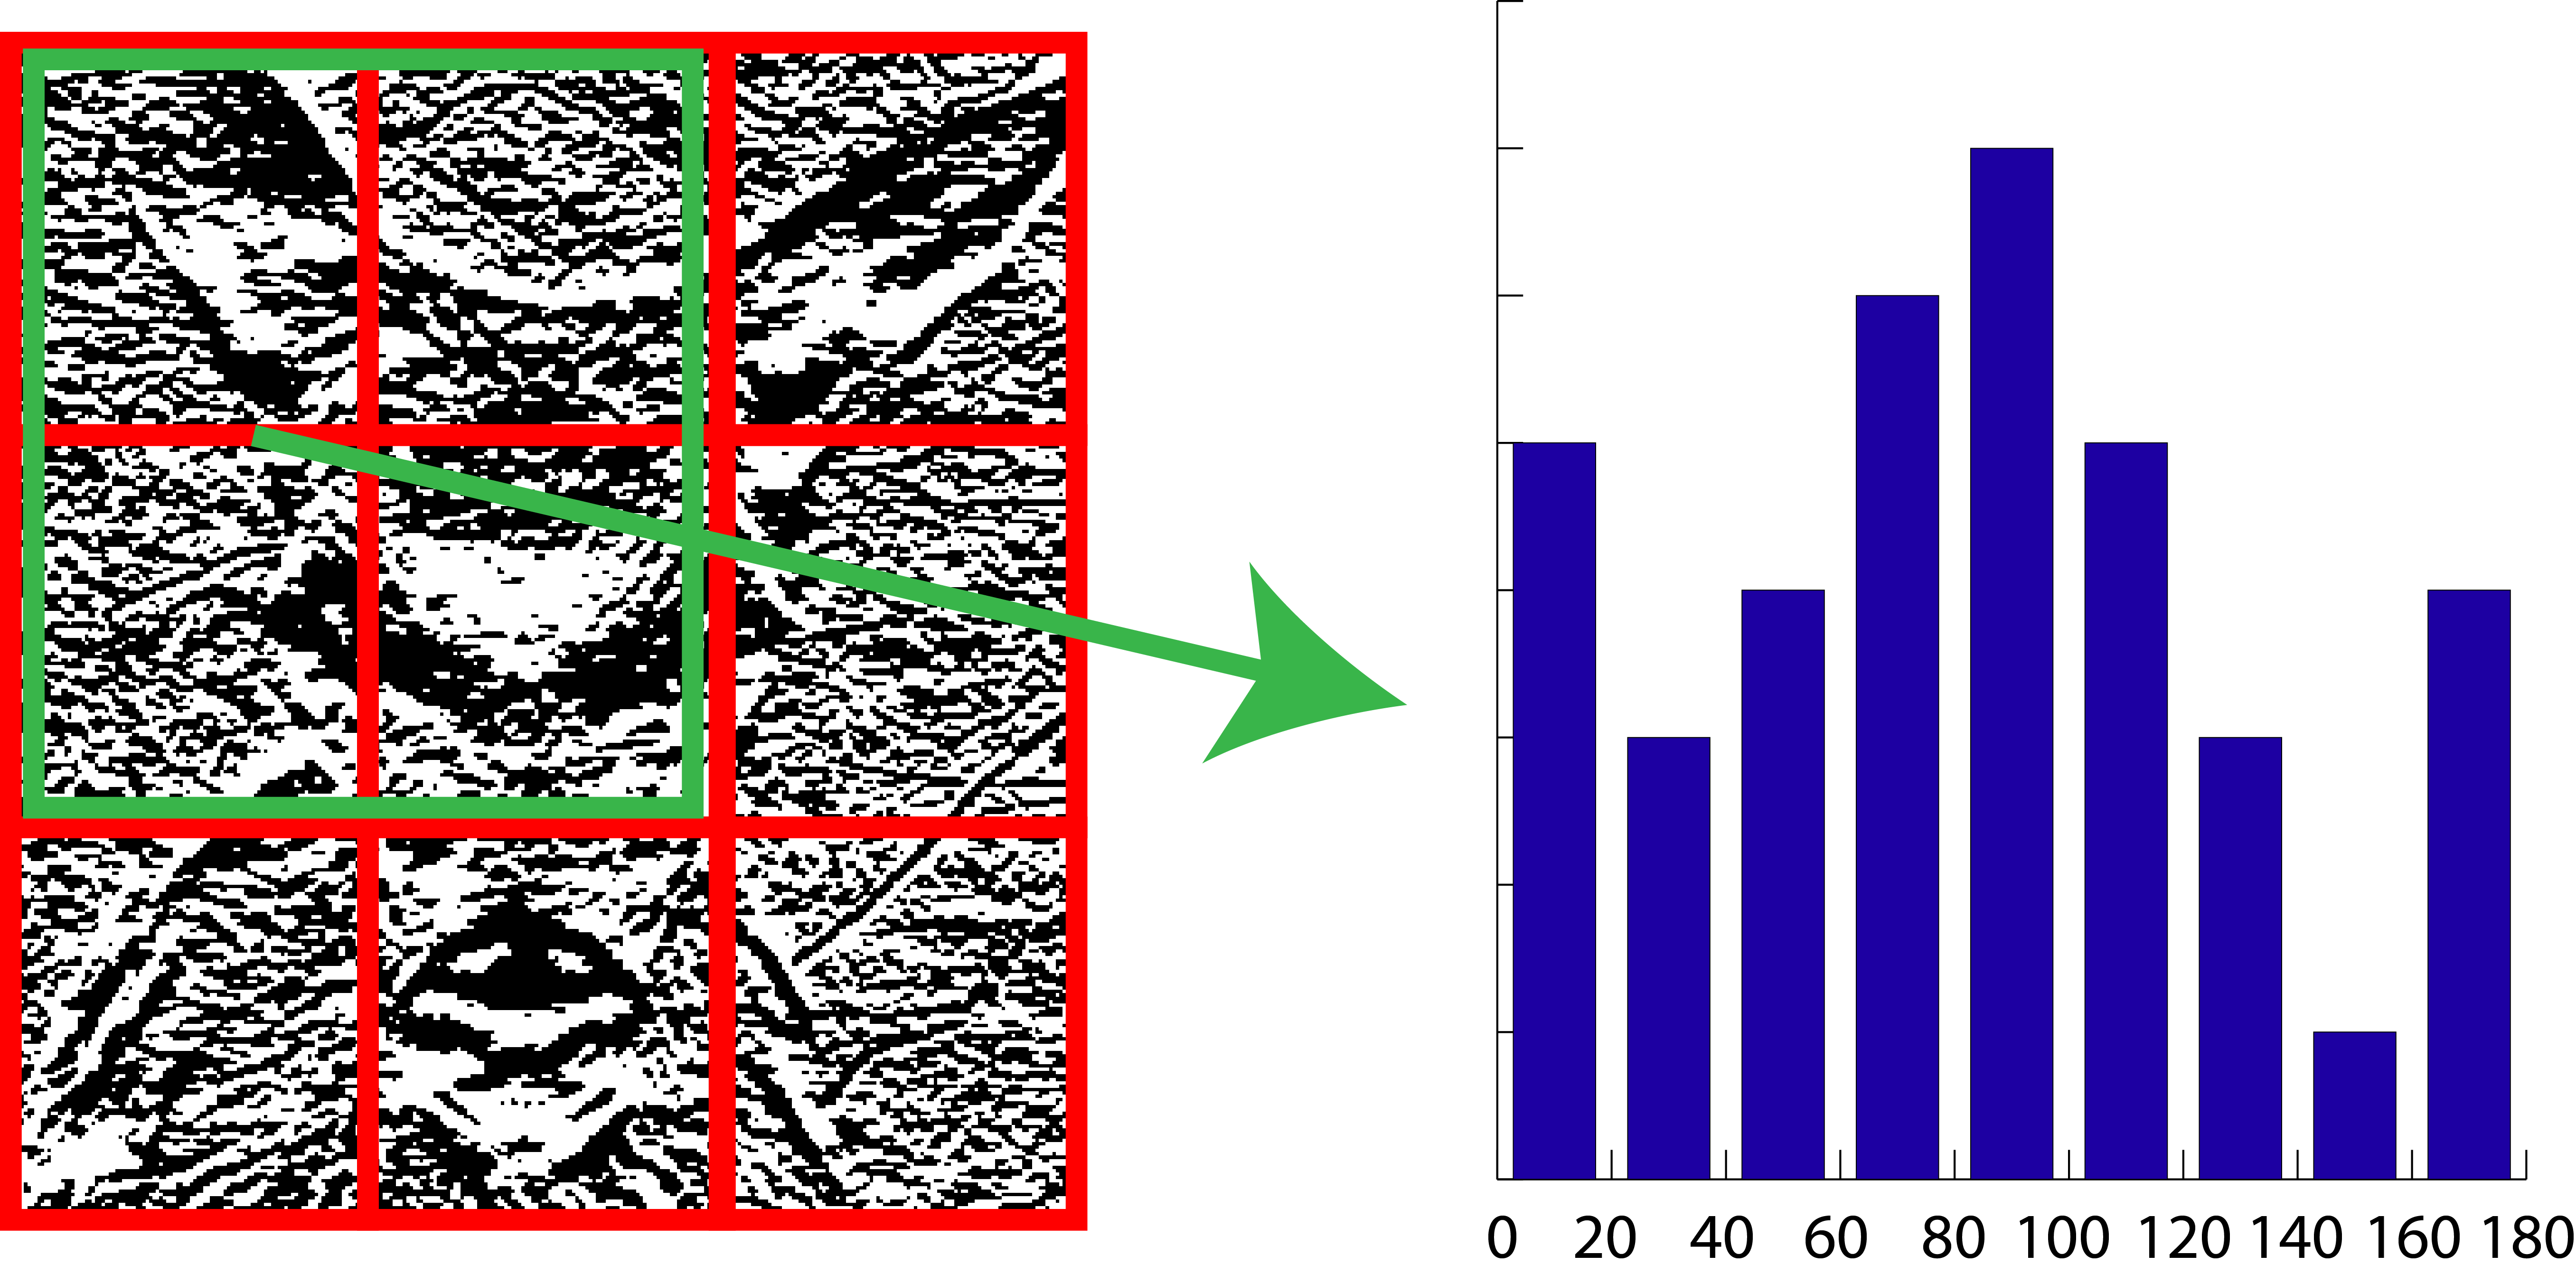
\includegraphics[trim={0 0cm 0cm 0cm},clip=true,width=13cm]{img/sobel2hog.png}
\end{tabular}
\captionof{figure}{Veranschaulichung der Erstellung eines HOG-Deskriptors. Das rote Raster visualisiert die Unterteilung in Zellen. Jeweils vier dieser Zellen werden zusammen als ein Block betrachtet. So das hier 4 Blöcke möglich wären. Für jeden Block wird dann ein normalisiertes Histogramm erstellt. Hier exemplarisch nur für den grünen Block gezeigt.}
\label{fig:sobel2hog}
\end{center}

\begin{center}
\begin{tabular}{c}
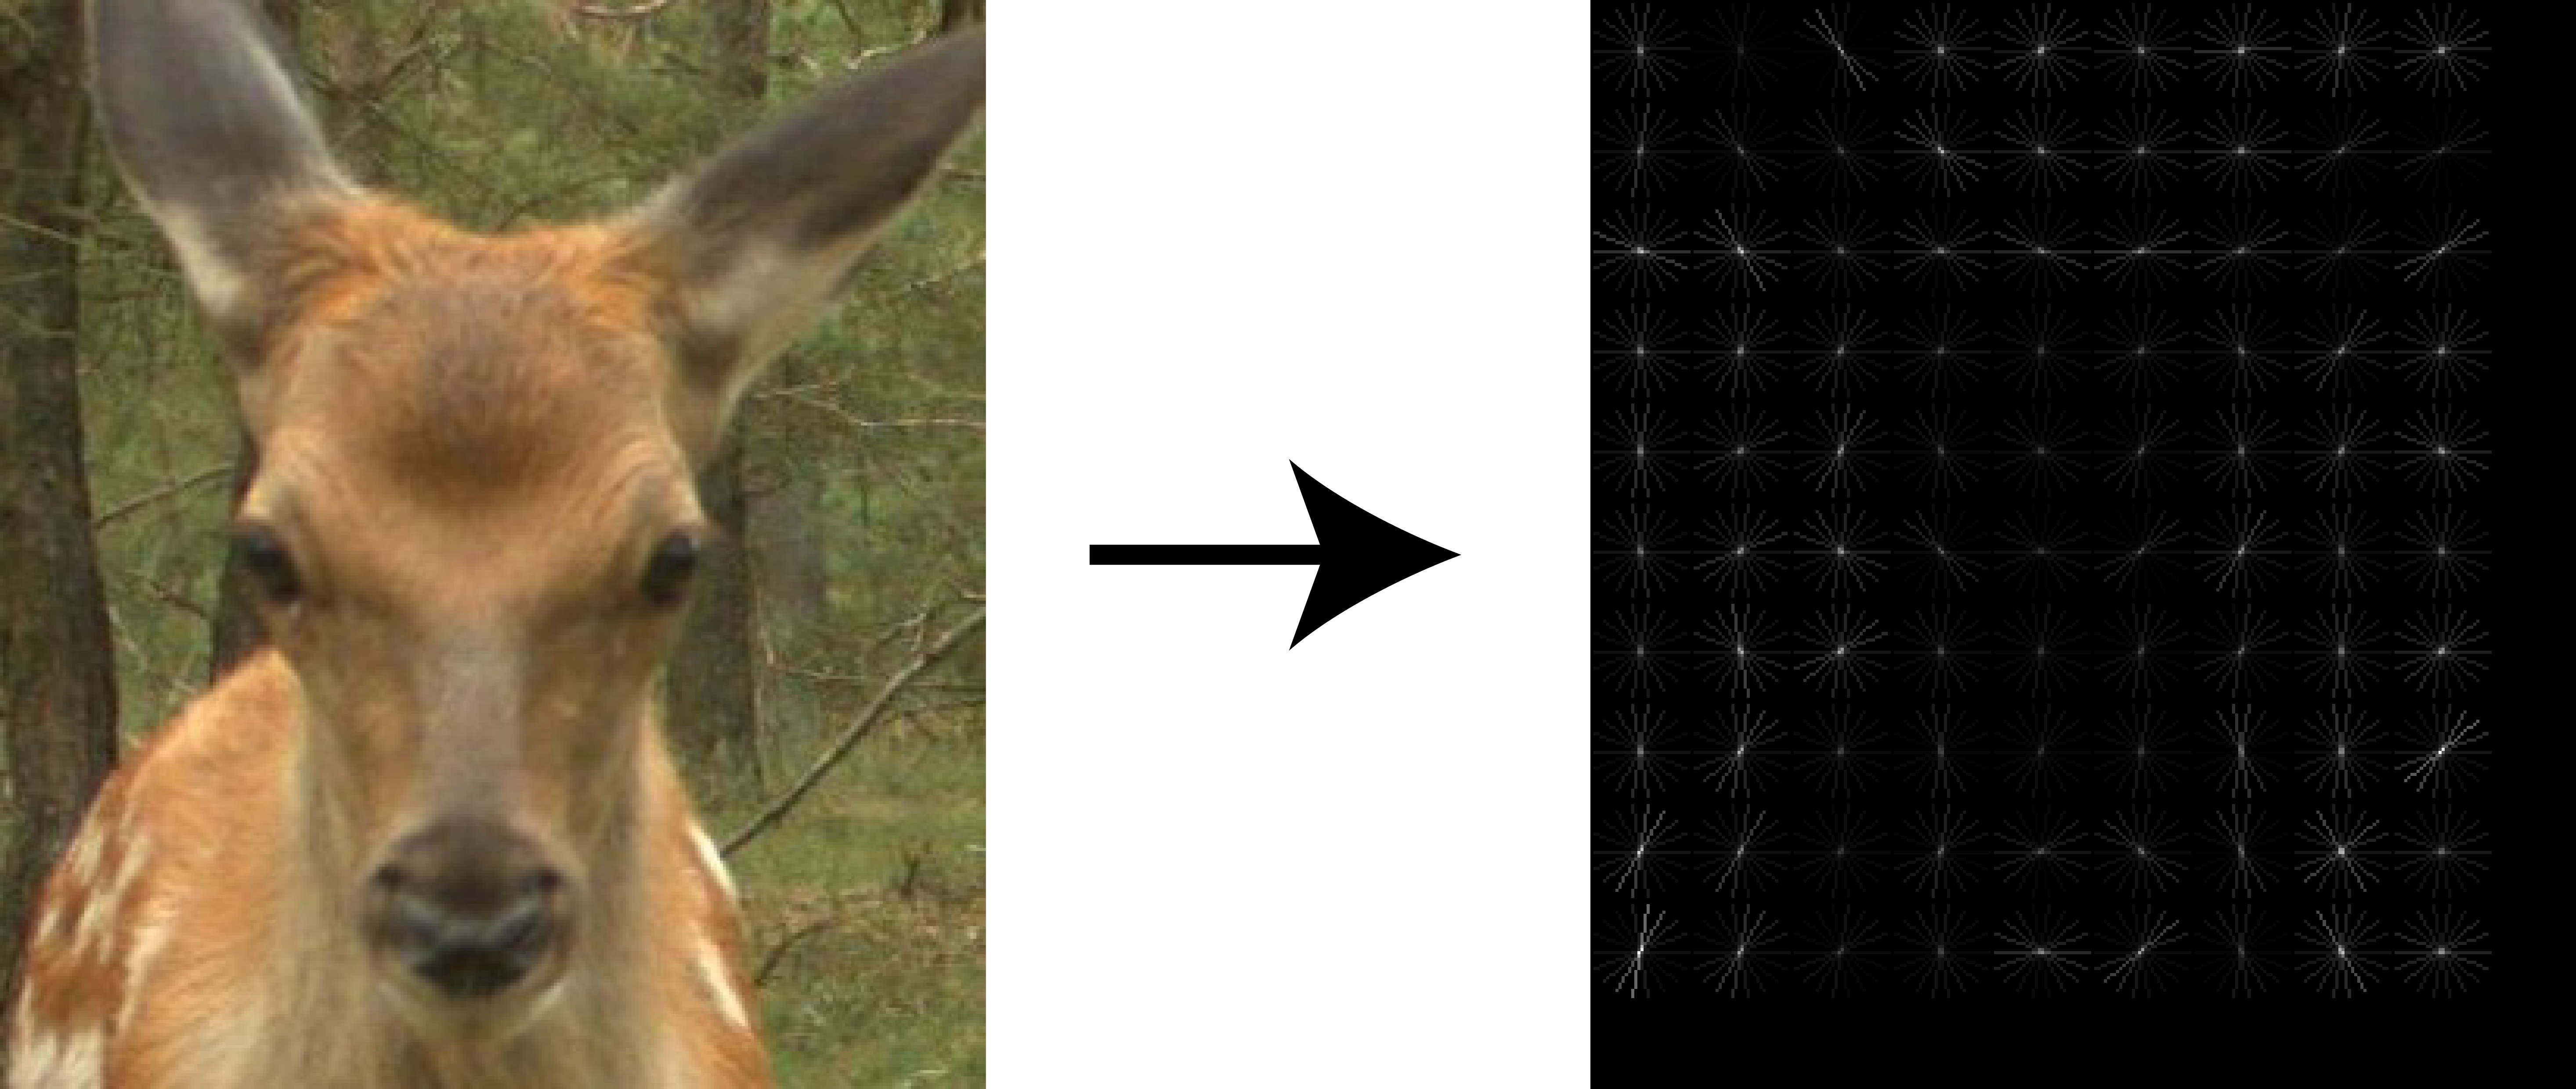
\includegraphics[trim={0 0cm 0cm 0cm},clip=true,width=13cm]{img/Img2HOG.png}
\end{tabular}
\captionof{figure}{Exemplarischer Bildausschnitt (links) und die visuell aufbereitet Repräsentation als HOG-Deskriptor (rechts). In der HOG Repräsentation ist es immer noch möglich das Reh zu erkennen.}
\label{fig:img2HOG}
\end{center}


\subsection{Technische Umsetzung der Klassifizierung} \label{ssec:implementation}
Umgesetzt wurde der HOG basierte Klassifizierer in Python mit OpenCV (Version: opencv-contrib-python 3.4.2.17). Der Klassifizierer setzt voraus, dass Bilder und die interessanten Regionen (ROI) bereits bestimmt wurden. Details zur ROI Bestimmungen werden in Kapitel~\ref{sec:PCA} gegeben. Eine Übersicht der Arbeitsweise wird in Abbildung~\ref{fig:hog_classification_ov} gezeigt. Dabei gibt es zwei Phasen: 1. Training und 2. Klassifikation. Die Trainings Phase wird durch den oberen Verlauf in der Abbildung skizziert. Dazu werden aus einem gelabeltem Bilderdatensatz deren relevanten ROIs selektiert. Für jedes ROI dieser Bilder wird wie in Abschnitt~\ref{ssec:intro_HOG} erklärt ein HOG-Deskriptor berechnet. Dabei wurde darauf geachtet, dass jedes ROI das selbe Seitenverhältnis besitzt. Zur Beschleunigung der Berechnung wurden die ROIs nur als Graustufenbilderverarbeitet und auf eine Größe von 64 x 128 Pixel² skaliert. Eine Zelle wurde auf 16 x 16 Pixel festgelegt, so das eine Block Größe von 32 x 32 Pixel² verwendet wurde. Diese Parameter wurden gewählt, das sie die experimentell bestimmten besten Ergebnisse lieferten (siehe Kapitel~\ref{sssec:HOG:parmeter}). Außerdem wurden die Orientierungen in 9 Gruppen sortiert, so dass eine richtungsunabhängige Orientierung betrachtet wurde. Sonstige Parameter des HOG-Deskriptors wurden auf den entsprechenden Standardwerten der OpenCV Implementierung belassen. 

Diese Deskriptoren sollen mit einer Support Vektor Maschine (SVM) trainiert und später klassifiziert werden. Dazu wurde die von OpenCV zur verfügungestellte Implementierung einer SVM verwendet. Für den Kernel der SVM wurde eine Radiale Basisfunktion als gewählt. Experimentell wurden die Parameter $C = 12,5$ und $\gamma = 0,50625$ als optimal bestimmt. Details zur Parameterwahl werden im Kapitel~\ref{sssec:HOG:parmeter} beschrieben.
Mit Hilfe der so trainierten SVM kann dann in der 2. Phase die Klassifikation der Bilder durchgeführt werden. Dazu werden analog für Bildausschnitte der Testdaten Feature Deskriptoren berechnet und diese von der SVM klassifiziert. Die Qualität dieser Klassifizierung wird im folgendem Unterkapitel beschrieben.
\begin{center}
\begin{tabular}{c}
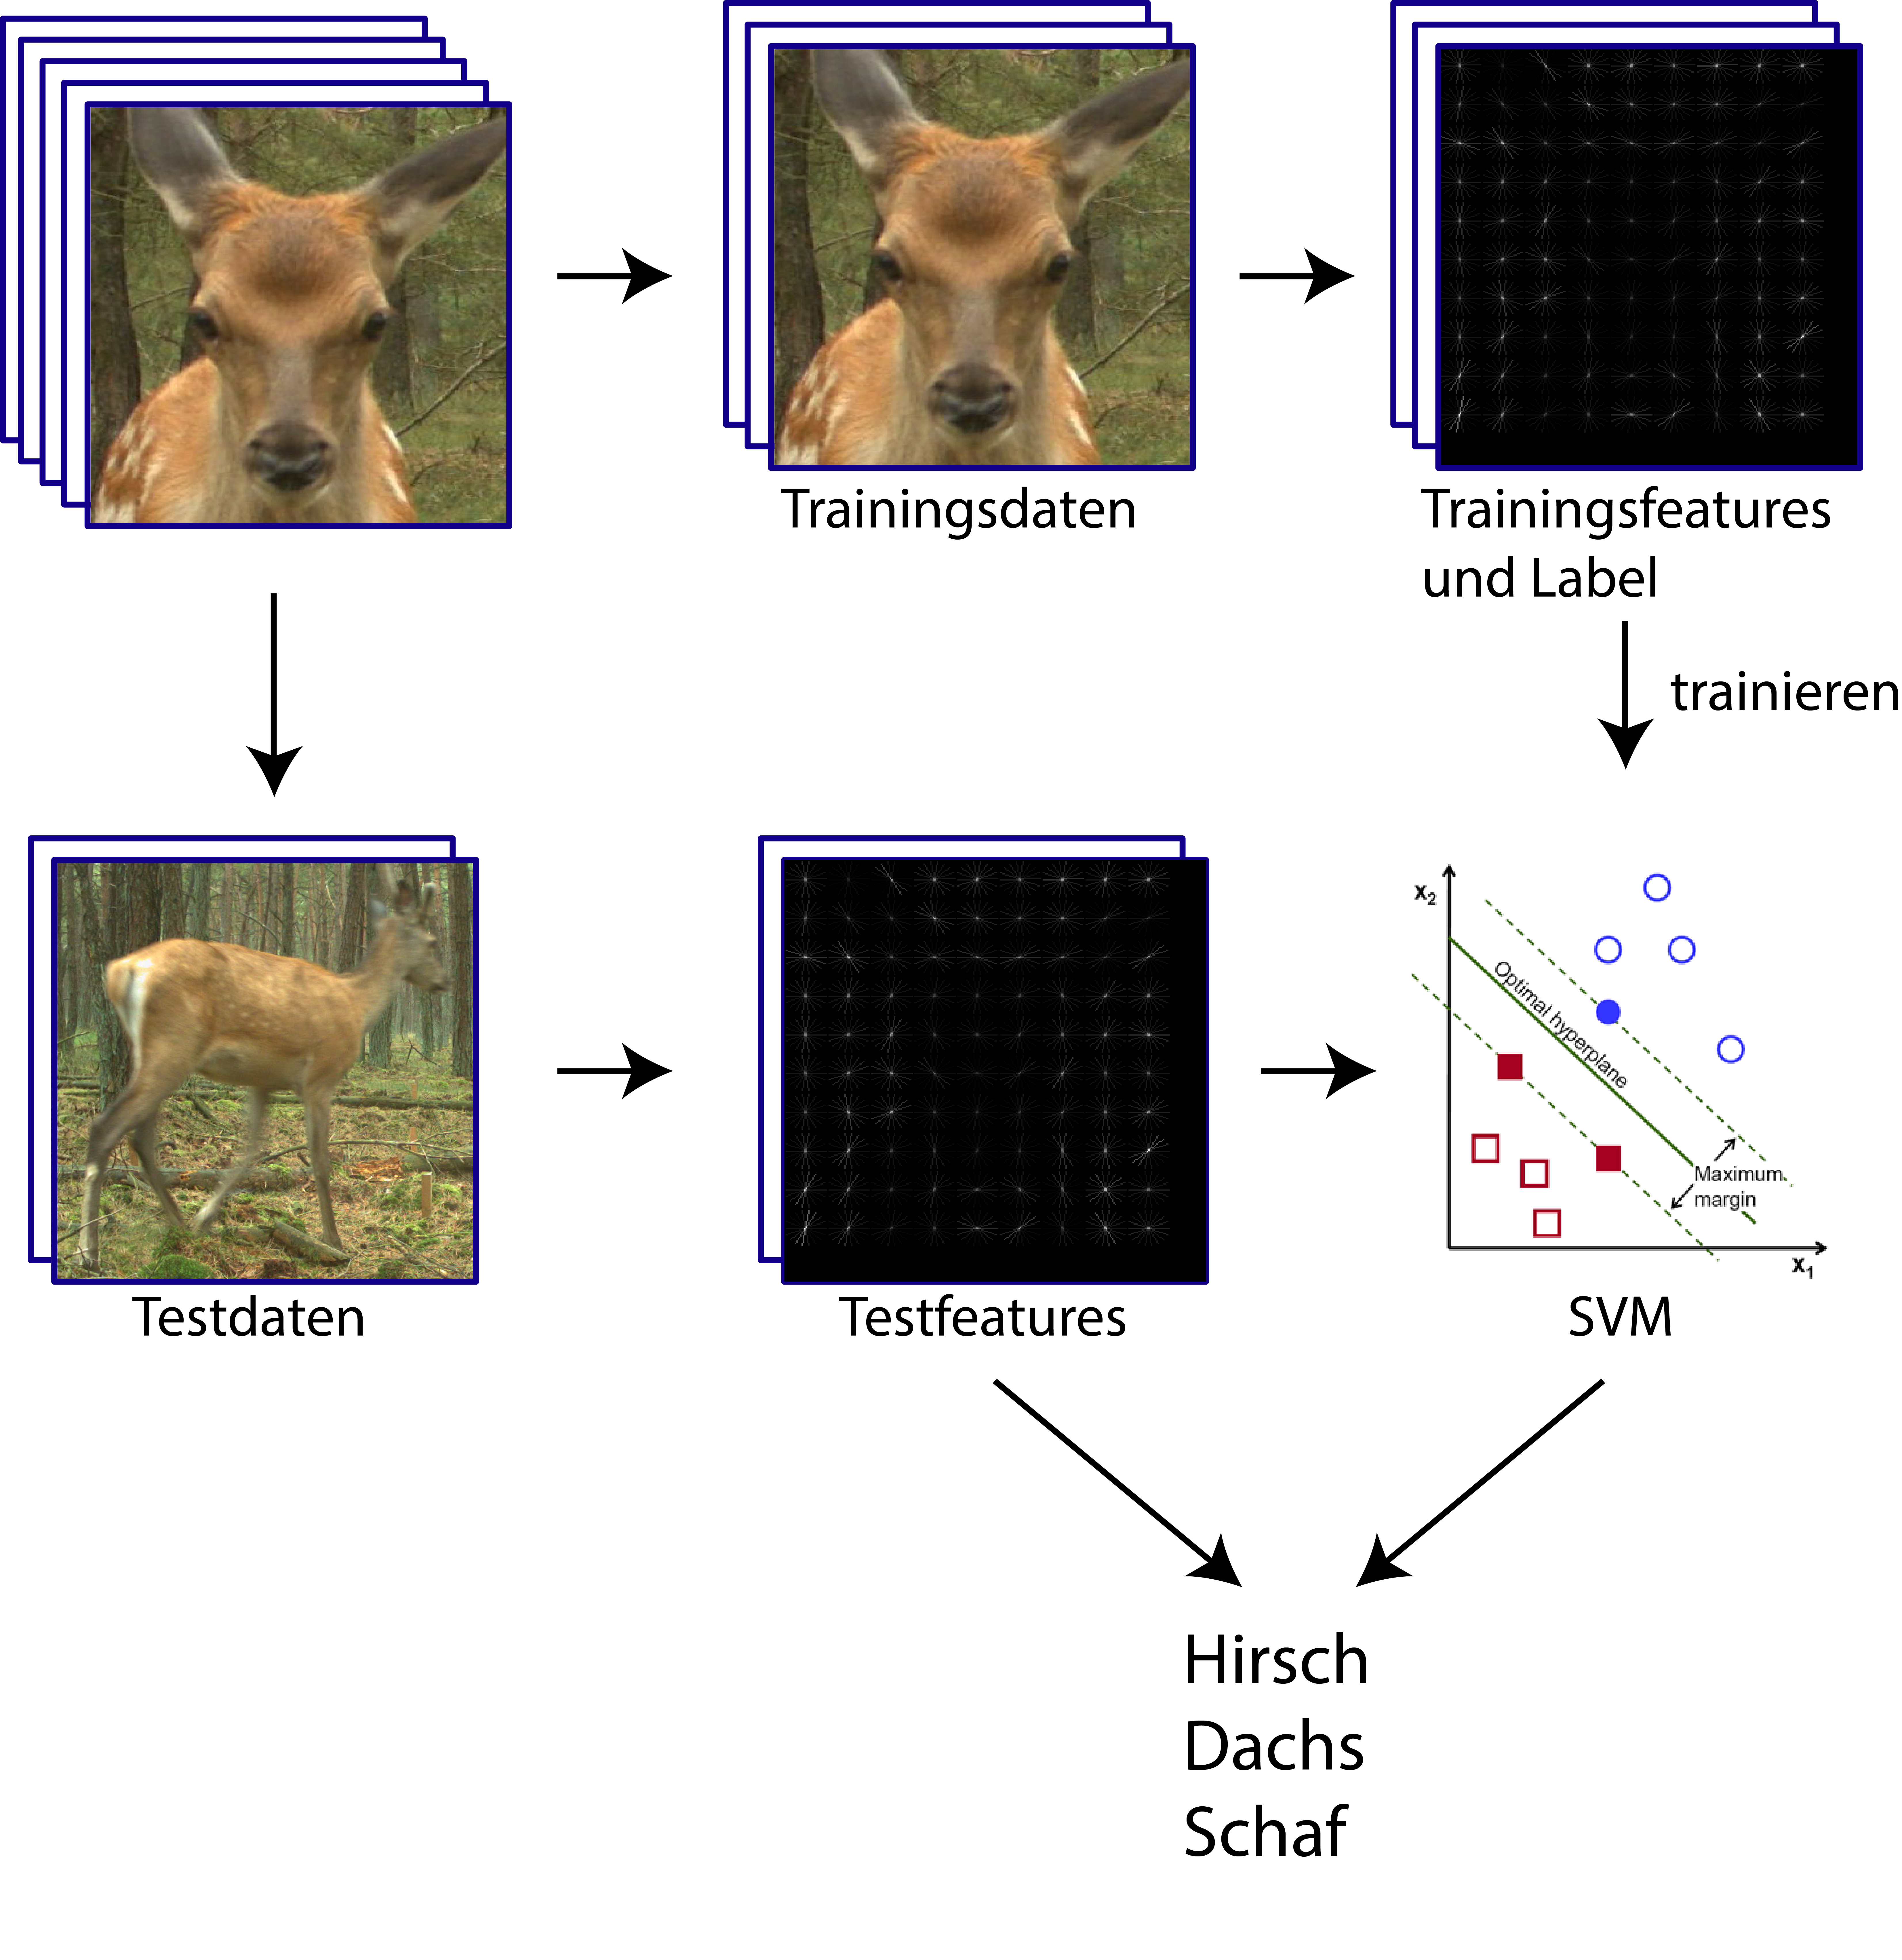
\includegraphics[trim={0 0cm 0cm 0cm},clip=true,width=13cm]{img/ClassificationOverview.png}
\end{tabular}
\captionof{figure}{Schaubild zur Klassifizierung mit einer SVM. Der obere Pfad repräsentiert die Trainingsphase und der untere Pfad die Russifizierungsphase. (Das SVM Bild (rechts unten) wurde aus der OpenCV Dokumentation übernommen \cite{SVM1})}
\label{fig:hog_classification_ov}
\end{center}


\subsection{Experimentelle Optimierung und Auswertung} \label{sec:HOG_parameter_and_results}
In diesem Kapitel wird die experimentelle Bestimmung der besten Parameter für den HOG-Deskriptor und die SVM behandelt. Für diesen Teil wurden die Tagesbilder von Dachs und Damhirsch verwendet.


\subsubsection{Arten der Testdaten} \label{sssec:test_data_HOG}
Der HOG-Klassifizierer wurde auf eine Datenbank mit bereits bestimmten ROIs verwendet. In ersten Experimenten und zur optimalen Parameterbestimmung wurden Daten mit manuell selektierten ROIs verwendet. Diese wurde getan um einen möglichen Fehler durch die automatische ROI Selektion mit PCA auszuschließen. Später wurde die SVM jedoch mit automatisch selektierten ROIs trainiert und ebenfalls automatisch selektierte ROIs klassifiziert. 
Da der Datensatz der Dachs Bilder sehr gering war, wurde versucht die Trainingsdatenmenge durch vertikale Spiegelung der Bilddaten künstlich zu erhöhen. Auf 10 Testläufen wurde eine geringe Verbesserung der Ergebnisse bestimmt. Auch wenn diese Erhöhung nicht signifikant war und in seltenen Fällen eine Reduktion der Präzision verursachte, wurde die künstliche Testdaten Erhöhung für alle Tests im folgenden Teil angewandt. 

Ein weiteres Problem der geringen Dachs Daten menge war, dass bei prozentualer Selektion der Trainingsdaten der Großteil aus Damhirsch Bildern bestand. Wurde die SVM mit diesen unausgewogenen verteilung der Tierklassen trainiert konnte die SVM fast nur noch Damhirsche erkennen. Die Erkennungsrate für Dachse lag dabei bei unter 50~\%. Dieses Problem wurde dadurch gelöst, dass darauf geachtet wurde gleich große Mengen an Trainingsdaten zu verwenden. Durch diese Maßnahme wurde die Präzision mit geeigneten Parametern auf durchschnitt über 90~\% erhöhen.

\subsubsection{Parameterbestimmung HOG-Deskriptor und Support Vektor Maschiene} \label{sssec:HOG:parmeter}
Einer der wichtigsten Parameter des HOG-Deskriptors ist die Größe des betrachteten Bildausschnittes und die Einteilung in Zellen, denn diese Größen bestimmen zum einem die benötigte Rechenzeit, zum anderem wie viele Details des Bildausschnittes regional aufgelöst werden. Außerdem ergibt sich aus dieser Kombination die Dimension des Ergebnis-Vektors. Dieser hat wiederum Einfluss auf den Rechenaufwand der SVM. Ziel dieser ersten Parameterfindung was es, die Präzision der Klassifizierung zu maximieren. Dabei wurde besonders darauf geachtet, dass die Präzision für beide trainierten Klassen maximal wurde. Dazu wurden die folgenden Bildausschnittgrößen betrachtet: 64 x 128, 128  x 256, 64 x 64, 128 x 128, 128 x 64 und 256 x 128 Pixel². Jede dieser Größen wurde mit einer Zellgröße von 16 x 16 und 32 x 32 Pixeln getestet. Für die Blockgröße wurden jeweils die Kombination aus 4 Zellen verwendet. Die Ergebnisse sind in Tabelle~\ref{tab:HOG_parameter_selection} gezeigt.  
Ebenfalls wurde versucht die Parameter der SVM zu optimieren. Dazu wurde die \textit{trainAuto} Methode von OpenCV verwendet. Die besten Parameter waren für die Kostenfunktion $C=12,5$ und $\gamma=0,50625$. Diese Werte liegen sehr nah an den Standard Werten ($C=12$ und $\gamma=0,5$) für die SVM. So das keine nennenswerten Änderungen an den Werten aus Tabelle~\ref{tab:HOG_parameter_selection} bestimmt werden konnten.

\begin{table}[]
\centering
\caption{Präzision der Klassifizierung abhängig von der Bildausschnittgröße und der Zellgröße. Es werden aus 50 Zufällig generierten Trainings- und Testdaten Reihenfolgen die jeweils erreichte durchschnittliche Präzision $\overline{p}$, die minimale sowie maximale erhaltene Präzision ($p_{min}, p_{max}$) und die Standardabweichung $\sigma$ angegeben. }
\label{tab:HOG_parameter_selection}
\begin{tabular}{cl}
\hline
\textbf{Ausschnitt [Pixel²]} & \multicolumn{1}{c}{\textbf{Zellgröße 16 x 16}}                                                                                                                                                  \\ \hline
\textbf{64 x 128}                         & \begin{tabular}[c]{@{}l@{}}Dachs: $\overline{p}= 0.913, p_{min}=0.750, p_{max}=1.000, \sigma=0.062$ \\ Damhirsch: $\overline{p}=0.914, p_{min}=0.831, p_{max}=0.987, \sigma=0.034$\end{tabular} \\
\textbf{128 x 256}                      & \begin{tabular}[c]{@{}l@{}}Dachs: $\overline{p}=0.488, p_{min}=0.167, p_{max}=0.833, \sigma=0.161$ \\ Damhirsch: $\overline{p}=0.996, p_{min}=0.949, p_{max}=1.000, \sigma=0.011$\end{tabular}          \\
\textbf{64 x 64}                           & \begin{tabular}[c]{@{}l@{}}Dachs: $\overline{p}=0.908, p_{min}=0.833, p_{max}=1.000, \sigma=0.045 $\\ Damhirsch: $\overline{p}=0.859, p_{min}=0.797, p_{max}=0.916, \sigma=0.035$\end{tabular}          \\
\textbf{128 x 128}                      & \begin{tabular}[c]{@{}l@{}}Dachs: $\overline{p}=0.818, p_{min}=0.500, p_{max}=1.000, \sigma=0.111 $\\ Damhirsch: $\overline{p}=0.951, p_{min}=0.882, p_{max}=0.992, \sigma=0.023$\end{tabular}          \\
\textbf{128 x 64}                        & \begin{tabular}[c]{@{}l@{}}Dachs: $\overline{p}=0.933, p_{min}=0.833, p_{max}=1.000, \sigma=0.050 $\\ Damhirsch: $\overline{p}=0.881, p_{min}=0.709, p_{max}=0.979, \sigma=0.069$\end{tabular}          \\
\textbf{256 x 128}                      & \begin{tabular}[c]{@{}l@{}}Dachs: $\overline{p}=0.675, p_{min}=0.250, p_{max}=1.000, \sigma=0.308 $\\ Damhirsch: $\overline{p}=0.781, p_{min}=0.367, p_{max}=1.000, \sigma=0.249$\end{tabular}          \\ \hline
 & \\
\hline
\textbf{Ausschnitt [Pixel²]} & \multicolumn{1}{c}{\textbf{Zellgröße 32 x 32}}                                                                                                                                                  \\ \hline
\textbf{64 x 128}                         & \begin{tabular}[c]{@{}l@{}}Dachs: $\overline{p}= 0.875, p_{min}=0.750, p_{max}=1.000, \sigma=0.067$ \\ Damhirsch: $\overline{p}=0.854, p_{min}=0.755, p_{max}=0.907, \sigma=0.044$\end{tabular} \\
\textbf{128 x 256}                      & \begin{tabular}[c]{@{}l@{}}Dachs: $\overline{p}=0.883, p_{min}=0.750, p_{max}=1.000, \sigma=0.076$ \\ Damhirsch: $\overline{p}=0.894, p_{min}=0.810, p_{max}=0.928, \sigma=0.037$\end{tabular}          \\
\textbf{64 x 64}                           & \begin{tabular}[c]{@{}l@{}}Dachs: $\overline{p}=0.975, p_{min}=0.917, p_{max}=1.000, \sigma=0.038 $\\ Damhirsch: $\overline{p}=0.859, p_{min}=0.708, p_{max}=0.574, \sigma=0.072$\end{tabular}          \\
\textbf{128 x 128}                      & \begin{tabular}[c]{@{}l@{}}Dachs: $\overline{p}=0.908, p_{min}=0.667, p_{max}=1.000, \sigma=0.102 $\\ Damhirsch: $\overline{p}=0.840, p_{min}=0.705, p_{max}=0.903, \sigma=0.062$\end{tabular}          \\
\textbf{128 x 64}                        & \begin{tabular}[c]{@{}l@{}}Dachs: $\overline{p}=0.967, p_{min}=0.917, p_{max}=1.000, \sigma=0.041 $\\ Damhirsch: $\overline{p}=0.834, p_{min}=0.776, p_{max}=0.932, \sigma=0.045$\end{tabular}          \\
\textbf{256 x 128}                      & \begin{tabular}[c]{@{}l@{}}Dachs: $\overline{p}=0.892, p_{min}=0.833, p_{max}=1.000, \sigma=0.075 $\\ Damhirsch: $\overline{p}=0.867, p_{min}=0.797, p_{max}=1.000, \sigma=0.954$\end{tabular}          \\ \hline
\end{tabular}
\end{table}

In den gezeigten Tabellen wird deutlich, dass die Präzision für die beiden Zellgößen in einem ähnlichem Genauigkeitsbereich liegt. Jedoch scheint eine größere Zellgröße etwas besser geeignet um Dachse zu erkenn und etwas schlechter geeignet um Damhirsche zu erkennen. Die besten Ergebnisse wurden für dir Kombination aus einer Bildauschnittgröße von 64 x 128 Pixel² und einer Zellgröße von 16 x 16 Pixel² erhalten. Dieser Wert entspricht den üblichen Standard Werten für die Fußgänger Detektion in OpenCV. Dies entspricht aber nicht der Erwartung bei der Tierdetektion, da die Seitenverhältnisse der betrachteten Tiere eher 1:1 bzw. 1:2 entsprechen. Eine Begründung für diese Abweichung kann an dieser Stell nicht gegeben werden. 

Im folgenden werden Experimente nur noch mit den hier gefundenen optimalen Parametern durchgeführt.

\subsubsection{Ergebnisse}
Die in Kapitel~\ref{sssec:HOG:parmeter} bestimmten optimalen Parameter wurden mit denen durch PCA bestimmten ROIs und der künstlichen Erhöhung der Testdaten getestet. Die in Tabelle~\ref{tab:HOG:ResultsAuto} gezeigten Ergebnisse stammen aus 50 Tests mit den selben Daten aber einer zufälligen Unterteilung der Daten in Trainings- und Testdaten. Es ist zu erkennen, das die Präzision etwas geringer ist als mit den manuell ausgewerteten ROIs. Dies war zu erwarten, da die automatische Bestimmung der ROIs mit PCA kleine Fehler enthält. Der Vorteil dieser Variante ist dennoch die automatische ROI selektion und damit eine deutliche Aufwandsreduktion für den Benutzer. 

\begin{table}[]
\centering
\caption{Präzision des Klassifizierers der sowohl mit den aus PCA stammenden ROIs trainiert und getestet wurde. Es werden aus 50 Zufällig generierten Trainings- und Testdaten Reihenfolgen die jeweils erreichte durchschnittliche Präzision $\overline{p}$, die minimale sowie maximale erhaltene Präzision ($p_{min}, p_{max}$) und die Standardabweichung $\sigma$ angegeben. }
 \label{tab:HOG:ResultsAuto}
\begin{tabular}{cl}
\hline
\textbf{Tiergattung} 	       & \multicolumn{1}{c}{\textbf{Präzision}}                                                                                                                                                  \\ \hline
\textbf{Dachs}                         &$\overline{p}= 0.859, p_{min}=0.761, p_{max}=0.957, \sigma=0.052$ \\
\textbf{Damhirsch}                &$\overline{p}=0.833, p_{min}=0.763, p_{max}=0.930, \sigma=0.032$ \\
\hline
\end{tabular}
\end{table}

Experimentell wurde der HOG-Klassifizierer auch auf eine Datenbank mit Damhirsch, Dachs, Wildschein und Schaf Bildern angewendet. Mit Erhöhung der Datenklassen wurde aber die Präzision der einzelnen Klassen wesentlich geringer. Der Wert lag üblicherweise unter 70~\%, für Dachse sogar unter 50~\%.



